\documentclass[12pt,a4paper,spanish]{book}
\usepackage[spanish]{babel}
\usepackage{amsmath}
\usepackage{graphicx}             
\usepackage{amsfonts}
\usepackage{amssymb}
\usepackage{graphics}
\usepackage{indentfirst}
\usepackage{enumerate}
\usepackage{fancyhdr}
\usepackage{fancybox}
\usepackage{lastpage}
\usepackage{color}
\usepackage{amsbsy}
\usepackage{amsthm}
\usepackage{listings}
\usepackage{titlesec}
\usepackage{titletoc}

\usepackage{makeidx}%glosario de términos
\usepackage[all]{xy}

\theoremstyle{definition}
\newtheorem{defi}{Definición}[section]

\theoremstyle{definition}
\newtheorem{propo}{Proposición}[section]

\theoremstyle{definition}
\newtheorem{coro}{Corolario}[section]

\usepackage{srcltx}%permite la busqueda inversa, si no viene por defecto en la version de LaTeX usada.

% lo siguiente solo usarlo cuando compilo directamente en pdflatex
% si lo uso compilando en latex el {\'\i}ndice no lo hace bien
\usepackage{hyperref}

\hypersetup{colorlinks=true, linkcolor=black, urlcolor=black, citecolor=black}
\hypersetup{bookmarksopen=false, bookmarksnumbered=true} \hypersetup{pdfstartview=FitH}

\makeindex


\setlength{\parskip}{5pt plus 2pt minus 1pt}
%%%%%%%%%%%%%%%%
%%% MACROS
%%%%%%%%%%%%%%%%

\newcommand{\cplx}[1]{{{\mathcal #1}^{\scriptscriptstyle\bullet}}}

\newcommand{\dmc}[1]{{D}^-(#1)}
\newcommand{\dbc}[1]{{D}^b(#1)}

\newcommand{\fmf}[3]{{\Phi^{#1}_{{\scriptscriptstyle #2\!\rightarrow\! #3}}}}
\newcommand{\lotimes}{{\,\stackrel{\mathbf L}{\otimes}\,}}

\newcommand{\cO}{{\mathcal O}}
\newcommand{\cP}{{\mathcal P}}
\newcommand{\cE}{{\mathcal E}}
\newcommand{\cG}{{\mathcal G}}
\newcommand{\calL}{{\mathcal L}}
\newcommand{\cI}{{\mathcal I}}
\newcommand{\cF}{{\mathcal F}}
\newcommand{\cQ}{{\mathcal Q}}
\newcommand{\cM}{{\mathcal M}}

\newcommand{\f}{\mathfrak{f}}

\newcommand{\iso}{{\,\stackrel {\textstyle\sim}{\to}\,}}
\newcommand{\what}[1]{{\widehat #1}}

\newcommand{\rk}{\operatorname{rk}}
\newcommand{\ch}{\operatorname{ch}}
\newcommand{\Td}{\operatorname{Td}}
\begin{document}

	\begin{titlepage}

    \begin{center}

        \vspace{0.75 cm}

        {\large\textbf{Universidad de Salamanca}\\
                        Grado en Matemáticas\\}

     \vspace{2cm}
         
        \rule[1mm]{400.0pt}{1mm}

        {\Large\textbf{
            REVISIÓN DE MÉTODOS MULTIVARIANTES\\
            SUPERVISADOS Y NO SUPERVISADOS\\
            \rule[1mm]{400.0pt}{1mm}\\
        \vspace{2cm}
             Trabajo Fin de Grado}}\\

        \vspace{1cm}
        
        \begin{figure}[h!]
            \begin{center}
              
\includegraphics[scale=.7]{Documentos Extra/escudo2tintas.pdf}\\
            \end{center}
		\end{figure}

		\vspace{0.75 cm}
		
        {\large\textbf{Alumno: Pedro Ángel Fraile Manzano }}

	\vspace{0.25 cm}
	{\large
	 \textbf{Tutoras: Ana Belén Nieto Librero y Nerea González García}} 
	 
	\vspace{0.5 cm}
	{\large
	 {Salamanca, Julio de 2023}} 

\end{center}

\end{titlepage}



	\pagenumbering{roman}
	\tableofcontents
	
	\addcontentsline{toc}{chapter}{Introducción}
\chapter*{Introducción}

\section{Distribuciones Multivariantes}
\begin{defi}
Un vector aleatorio \textbf{X} es $\ldots$ %%@todo
\end{defi}
	
	
	\input{Métodos supervisados.tex}
	
	%\input{Documentos Extra/Conceptos Básicos.tex}
	
	\chapter{Análisis de Componentes Principales}
\section{Introducción}

\noindent Sea una población de la que se han tomado $n$ muestras de las cuales hemos medido $p$ variables. Del conjunto de datos que resulta, podemos dar la matriz de datos $\mathbf{X}$ de tamaño $n\times p$. 

En consecuencia, las muestras $y_i$, con $i=1\ldots n$ se pueden interpretar como elementos de $\mathbb{R}^p$, pero si $p>3$, la representación gráfica de estos datos no se puede realizar

El análisis de componentes principales, aunque normalmente se utiliza con el objetivo de representar los datos de manera sencilla, también podría llegar a ser útil en la reducción de la dimensionalidad para evitar el overfitting en el aprendizaje automático. 

Este método es una técnica matemática que dado un vector aleatorio $\textbf{X}^T=[X_1,\ldots X_p]$, con vector de media $\mu$ y matriz de covarianzas $\Sigma$, utiliza transformaciones ortogonales para conseguir las componentes principales. 

Estas componentes principales son combinaciones lineales de las variables que forman el vector, de manera que estando correladas las iniciales, las componentes no lo están y se busca calcularlas con la máxima varianza posible. 

Esta transformación se busca ya que si varias variables están altamente correladas, entonces están aportando la misma información, siempre que no sean dependientes. Podemos encontrar por esta razón variables que no estén correladas, lo que implica que no dan la misma información y que en consecuencia pueden aportar mayor información acerca de la variación de los datos, sin tener que ser compartida o repetida por varias variables. 

Al finalizar este Análisis de Componentes Principales, obtendremos un conjunto de variables nuevas no correladas entre sí, que son combinación lineal de las iniciales que maximizan la varianza en cada paso.

Añadir que si las variables no están correladas o están cerca de no estarlo, el Análisis de Componentes Principales no tiene sentido ya que el conjunto de componentes principales será parecido a las variables iniciales, con la única diferencia que estarán ordenadas por orden creciente de varianza.  


\section{Definición y cálculo de las Componentes}

Sea un vector aleatorio $\textbf{X}^T=[X_1,\ldots X_p]$ con media $\mu$ y matriz de covarianzas $\Sigma$. 
\begin{defi}
Las componentes principales son combinaciones lineales de las variables $X_1 \ldots X_p$
\begin{equation}
\textbf{Y}_j=a_{1j}X_1+\ldots a_{pj}X_p=\textbf{a}_j^T\textbf{X}\quad 
\end{equation}

\noindent Donde $\textbf{a}_j$ es un vector de constantes y la variable $\textbf{Y}_j$ cumple lo siguiente:
\begin{itemize}
\item Si $j=1$ $Var(\textbf{Y}_1)$ es máxima restringido a $\textbf{a}_1^T \textbf{a}_1=1$
\item Si $j>1$ debe cumplir:
\begin{itemize}
\item $Cov(\textbf{Y}_j,\textbf{Y}_i)=0\quad \forall i<j $
\item $\textbf{a}_j^T \textbf{a}_j=1$
\item $Var(\textbf{Y}_j)$ es máxima. 
\end{itemize}

\end{itemize}

\end{defi}

\noindent El cálculo de la primera componente principal se lleva a cabo con un proceso de optimización de la función $Var(\textbf{Y}_1)$ sujeto a la restricción de que $\textbf{a}_1^T\textbf{a}_1=1$. Aplicando el método de los multiplicadores de Lagrange, dada una función $f(\textbf{x})=f(x_1\ldots x_p)$ diferenciable con una restricción $g(\textbf{x})=g(x_1\ldots x_p)=c$ entonces existe una constante $\lambda$ de manera la ecuación:
\begin{equation}
\dfrac{\partial f}{\partial x_i}-\lambda\dfrac{\partial g}{\partial x_i}=0 \quad i=1,\ldots p 
\end{equation}

\noindent Tiene como solución los puntos estacionarios de $f(\textbf{x})$

\newpage
Sea ahora la función $L(\textbf{x})= f(\textbf{x})-\lambda[g(x)-c]$  entonces podemos simplificar la expresión anterior a:
\begin{equation}
\dfrac{\partial L}{\partial \textbf{x}}=0
\end{equation}

\noindent En nuestro caso particular $L(\textbf{a}_1)=\textbf{a}_1^T \Sigma \textbf{a}_1 - \lambda[\textbf{a}_1^T \textbf{a}_1-1]$. Al derivarla obtenemos que :
\begin{align*}
\dfrac{\partial L}{\partial \textbf{a}_1} &= 2\Sigma \textbf{a}_1 - 2\lambda\textbf{a}_1\\
& = 2(\Sigma-\lambda)\textbf{a}_1 
\end{align*}

\noindent Igualando a 0 tenemos la siguiente ecuación: 
\begin{equation}
(\Sigma-\lambda I)\textbf{a}_1=0
\end{equation}

\noindent Para que la ecuación tenga una solución que no sea la trivial, tenemos que elegir $\lambda$ de manera que $|\Sigma-\lambda I| = 0$. Luego $\lambda$ es uno de los valores propios de la matriz. Generalmente una matriz $(p\times p)$ tiene $p$ valores propios $\lbrace\lambda_1, \ldots ,\lambda_p \rbrace$ y como $Var(\textbf{Y}_1)=Var(\textbf{a}_1^T\textbf{X})= \textbf{a}_1^T \Sigma \textbf{a}_1 =\textbf{a}_1^T \lambda \textbf{a}_1=\lambda$ que es la variable a maximizar, elegimos $\lambda=\max \lbrace\lambda_1, \ldots ,\lambda_p \rbrace$, por tanto, el vector $\textbf{a}_1$ es el vector propio con valor propio $\lambda=\lambda_1$ reordenando si es necesario.\\

\noindent Una vez calculada la primera componente principal $\textbf{Y}_1$, la segunda componente se calcula de manera análoga, maximizando $Var(\textbf{Y}_2)=Var(\textbf{a}_2^T\textbf{X})$ condicionada por $\textbf{a}_2^T\textbf{a}_2=1$. A esta restricción tenemos que añadir la restricción $Cov(\textbf{Y}_1,\textbf{Y}_2)=0 $

\begin{propo}
La condición $Cov(\textbf{Y}_1,\textbf{Y}_2)=0 $ equivale a la condición $\textbf{a}_2^T\textbf{a}_1 = 0$
\end{propo}
\begin{proof}
Utilizando que $\textbf{Y}_j=\textbf{a}_j^T \textbf{X}\quad \forall j$ , tenemos entonces que:
\begin{align*}
Cov(\textbf{Y}_2,\textbf{Y}_1)&= Cov (\textbf{a}_2^T\textbf{X},\textbf{a}_1^T\textbf{X})\\ 
&= E(\textbf{a}_2^T(\textbf{X}-\mu)(\textbf{X}-\mu)^T \textbf{a}_1)\\
&= \textbf{a}_2^T E((\textbf{X}-\mu)(\textbf{X}-\mu)^T) \textbf{a}_1\\
&= \textbf{a}_2^T \Sigma \textbf{a}_1 \\
&= \textbf{a}_2^T \lambda_1 \textbf{a}_1
\end{align*}
\noindent De manera que, si $a_2^T \lambda_1 a_1 = 0 \Rightarrow a_2^T a_1=0 $, luego son vectores ortogonales entre sí.
\end{proof}

\noindent \emph{Observación: } Esta proposición se puede extender de manera simple al caso de tener que calcular la $i$-ésima componente principal habiendo calculado las anteriores de las cuales sepamos sus valores propios. 

\begin{coro}
Las componentes principales son todas perpendiculares entre sí. 
\end{coro}



	
	
	%\section{Análisis de cluster}

\noindent Según Jain y Dubes  el análisis de \emph{cluster} es un conjunto de técnicas exploratorias que toman un conjunto de datos resultantes de recoger $N$ observaciones sobre $p$ medidas diferentes y buscan agrupar las observaciones. También se puede utilizar agrupaciones de variables pero no se desarrollará.

\noindent Para empezar, debemos definir que es un \emph{cluster}. Como en nuestro caso no buscamos agrupar variables, sino observaciones o mediciones, utilizaremos la definición dada en \cite{Everitt 2011}.

\begin{defi}
Diremos que un \emph{cluster} o conglomerado es un subconjunto de las observaciones que son similares entre sí. 
\end{defi}

\noindent Es fácil observar que los clusters definen la siguiente relación de equivalencia $\mathcal{R}$ en la que dos observaciones, $\mathbf{x}_i,\mathbf{x}_{i'}, i,i'=1, \ldots, N$ están relacionadas si pertenecen al mismo clúster \cite{Cuadras 2014}. Por tanto, cada \emph{cluster} genera una clase de equivalencia $[c_k], k=1\ldots K$ donde $K$ es el número de clusters

\noindent El conjunto de \emph{clusters} generan un \emph{clustering} o partición , es decir:
\begin{defi}
Se llama \textit{clustering} a la partición que provoca la relación $\mathcal{R}$ del espacio de observaciones. 
\end{defi}

\noindent Para llegar a dichas particiones podemos usar distintos tipos de algoritmos según el número de particiones distintas que se generen a lo largo del proceso \cite{Jain 1988}:
\begin{itemize}
\item Particional Son aquellos procesos de \emph{clustering} en los que de manera previa se conocen el número de \emph{clusters} y por tanto, se genera una partición que se va modificando.
\item Jerárquico, si el proceso genera una secuencia anidada de particiones, es decir, que dependiendo de cómo se desarrolle puede ser de los siguientes tipos:
\begin{itemize}
\item Aglomerativo Cuando se inicia con una partición que tiene $N$ \emph{clusters} con una observación en cada uno. Este tipo de algoritmos va tomando los \emph{clusters} y junta aquellos según un criterio establecido hasta llegar a un criterio de parada. 
\item Divisivo Cuando empieza con un único \emph{cluster} que contiene a las $N$ observaciones. En cada paso se va dividiendo los cluster siguiendo algún criterio hasta llegar al criterio de parada. 
\end{itemize}
\end{itemize}

\noindent En resumen, el análisis de cluster es un conjunto de técnicas que permiten la simplificación estructural de las observaciones recogidas de un vector aleatorio mediante la agrupación de las mismas en conjuntos llamados clusters \cite{Everitt 2011}. 

\noindent El análisis de clusters ha sido aplicado en infinidad de áreas como el marketing con el objetivo de segmentar los anuncios \cite{Okazaki 2006}, la psicología para detectar si se da un sólo trastorno en una población \cite{Everitt 2002} o en el caso de la medicina para intentar estudiar la supervivencia de pacientes con carcinoma renal \cite{Witten 2010}. Estos son ejemplos de unas pocas aplicaciones, pero también nos pueden ayudar en la predicción del riesgo crediticio, segmentación electoral etc... 

\subsection{Algoritmos jerárquicos}

\noindent Los algoritmos jerárquicos calculan en cada paso la similaridad o disimilaridad entre \emph{clusters} para generar nuevas particiones del espacio uniendo o separando los distintos \emph{clusters}.

\noindent Un algoritmo jerárquico genera una secuencia de particiones anidada que está definida de la siguiente manera \cite{Scitovski 2021} :
\begin{defi}
Una partición del espacio $\Pi^{(r)}$ está anidada en otra partición $\Pi^{(k)}$ y se denota $\Pi^{(r)} \sqsubset \Pi^{(k)}$ si cumple lo siguiente:
\begin{itemize}
\item El número de clusters de $\Pi^{(k)}$ es menor que el de $\Pi^{(r)}$. 
\item Cada cluster de la partición $\Pi^{(r)}$ es un subconjunto de algún cluster de $\Pi^{(k)}$. 
\end{itemize}
En el caso de un algoritmo aglomerativo tendremos que $k>r$, es decir en el paso $k$-ésimo el número de \emph{clusters}, es menor que en cualquier paso anterior.

\end{defi}

\noindent La pregunta que hay que hacer antes de aplicar este tipo de algoritmos, es cómo calcular las distancias o similaridad entre dos observaciones. Hay que distinguir dos casos, el cálculo inicial de las distancias entre observaciones del espacio y la distancia entre \emph{clusters}. Dependiendo de como se elijan sobre todo las últimas se tendrá un algoritmo de \emph{clustering} u otro \cite{Peña 2002}. 

\noindent En particular los métodos jerárquicos se pueden aplicar a distancias y similaridades, (veáse \cite{Mardia 1979}) Estas se pueden definir de distintas formas pero la más habitual es la distancia de Mahalanobis como se detallaba en la definición \ref{Mahalanobis}. Aunque esta sólo se detalla para variables continuas. 

\noindent Dependiendo de como se defina dicha distancia va a provocar que tengamos uno u otro tipo de algoritmo jerárquico.\cite{Everitt 2011, Johnson 2007, Peña 2002}
\begin{itemize}
\item El vecino más proximo: $d(C,C')=\min_{\mathbf{x}_i\in C, \mathbf{x}_{i'}\in C'}(\mathbf{x}_i,\mathbf{x}_{i'})$, es decir, se toma como la distancia entre los \emph{clusters} y una observación, $\mathbf{x}_{i'}$, el mínimo de las distancias entre las observaciones del propio cluster y la observación considerada.
\item El vecino más lejano: $d(C,C')=\max_{\mathbf{x}_i\in C, \mathbf{x}_{i'}\in C'}(\mathbf{x}_i,\mathbf{x}_{i'})$, es decir, se toma como la distancia máxima entre todas las posibles. 
\item Enlace medio \begin{equation}
d(C,C')=\dfrac{1}{N_C}\dfrac{1}{N_C'}\sum_{\mathbf{x}_i\in C}\sum_{\mathbf{x}_{i'}\in C'} d(\mathbf{x}_i, \mathbf{x}_{i'})
\end{equation}
donde $N_C, N_{C'}$ son el número de observaciones que hay en cada cluster. Es decir, es la media de todas las distancias. 
\item Ward:
\begin{equation}
d(C,C')=\dfrac{1}{N_C}\dfrac{1}{N_C'}\sum_{\mathbf{x}_i\in C}\sum_{\mathbf{x}_{i'}\in C'} (d(\mathbf{x}_i, \mathbf{x}_{i'}))^2
\end{equation} 

donde $N_C, N_{C'}$ son igual que antes. En particular, el algoritmo de Ward calcula las variación en los \emph{clusters}
\end{itemize}

\noindent En general, un algoritmo jerárquico aglomerativo funciona de la siguiente manera:

\begin{itemize}
\item Se inicia con una partición que tiene $N$ \emph{clusters} con una única observación cada uno.
\item Se calcula la matriz de distancias entre los \emph{clusters}. 
\item Se unen los dos clusters que menor distancia tengan entre ellos. De esta manera, se reduce el número de clusters en 1.  
\item Se repiten los dos pasos anteriores hasta tener un único cluster. 
\end{itemize}

\noindent El resultado de estos algoritmos es un dendograma \cite{Mardia 1979}
\begin{defi}
Un dendograma es un diagrama de árbol en el que en el eje horizontal se sitúan las observaciones mientras que en el eje vertical se representan las distancias. Cada nodo representa una unión de los clusters. 
\end{defi}

\noindent Los siguientes dendogramas \ref{fig:complete_linkage} \ref{fig:single_linkage}  son resultado de aplicar un algoritmo jerárquico al conjunto \emph{IRIS} de Fisher \cite{Iris Fisher}.
\begin{figure}[h]
 \centering
  \subfloat[Enlace completo]{
   \label{fig:complete_linkage}
    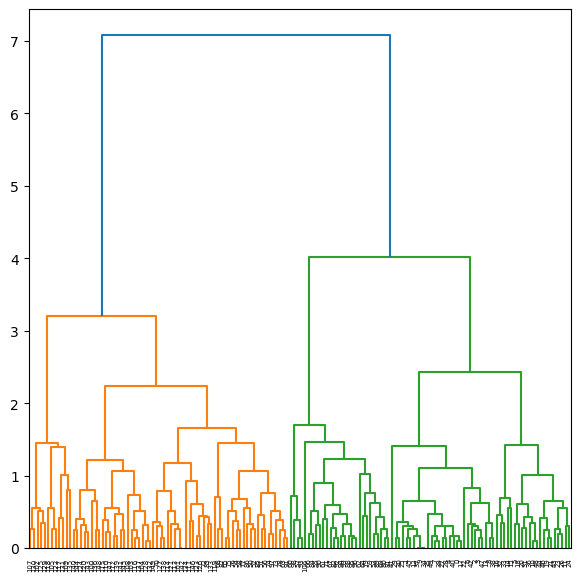
\includegraphics[width=0.3\textwidth]{Documentos Extra/Imagenes/complete_linkage.png}}
  \subfloat[Enlace simple]{
   \label{fig:single_linkage}
    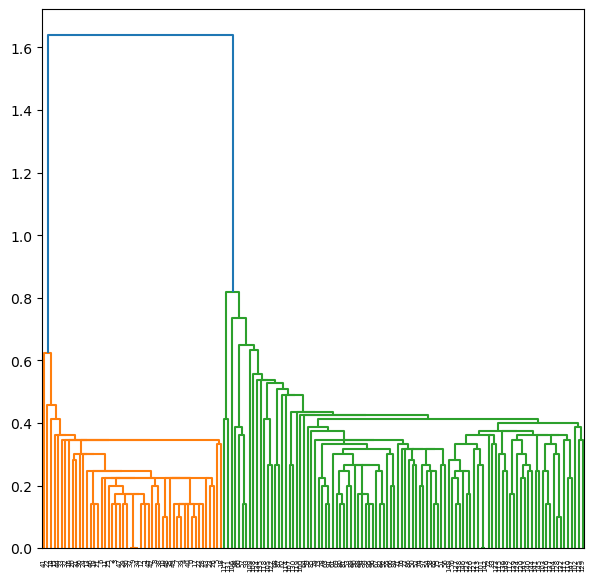
\includegraphics[width=0.3\textwidth]{Documentos Extra/Imagenes/single_linkage.png}}
 \caption{Diagramas obtenidos utilizando la biblioteca de Python Scikit-Learn}
 \label{fig:Dendogramas distintos enlaces }
\end{figure}
\newpage
\subsection{Algoritmos particionales}

\noindent Dada una matriz de datos $\mathbf{X}$ de tamaño $N\times p$ resultado de realizar $N$ observaciones de $p$ variables aleatorias. El \emph{clustering} particional busca hacer una partición que divida las observaciones en $K$ grupos homogéneos 

\begin{defi}
Se llama \emph{centroide} de un cluster $C_k,\quad k=1,\ldots,K$ al vector de tamaño $p$ cuyas componentes son las medias de cada una de las variables de todas las observaciones del \emph{cluster} $C_k$:
\begin{equation}
\overline{x}_{jk}=\dfrac{1}{|C_k|}\sum_{i\in C_k}  x_{ij} \quad \forall j=1,\ldots, p
\end{equation}
\end{defi}

\noindent El algoritmo de $K$-medias es el más importante de este tipo \cite{Johnson 2007}. Se desarrolla de la siguiente manera  :
\begin{enumerate}
\item Se asignan a cada una de las observaciones en cada uno de los $K$ \emph{clusters}. Se calculan los centroides de dichos \emph{clusters}.
\item Se comprueba la distancia euclídea de cada una de las observaciones a los centroides de los \emph{clusters} y se reasignan las observaciones de acuerdo al  más cercano. Tras esto se recalculan los centroides.
\item Se repiten los dos pasos anteriores hasta que las asignaciones no cambien. 
\end{enumerate}

\noindent Resaltar que este algoritmo tiene un problema y es que los resultados finales 

\noindent Hay otras alternativas que utilizan criterios de variabilidad intra grupos o entre grupos para realizar las asignaciones óptimas fijados el número de clusters, para profundizar en dicho enfoque, léase \cite{Everitt 2011, Peña 2002, Hartigan 1975}







	
	%
\begin{thebibliography}{99}
    \rhead[]{Bibliografía}
	
	\addcontentsline{toc}{chapter}{Bibliografía}

\bibitem{Chatfield 1989} \textbf{Chatfield,C y Collins A.J (1989)}. {\em Introduction to multivariate analysis}, Chapman and Hall.

\bibitem{Jollife 1986} \textbf{Jollife I.T.(1986)}. {\em Principal Component Analysis}, Springer-Verlag.

\bibitem{Hastie 2001} \textbf{Hastie, T.,Tibshirani, R. y Friedman J. (2001)}, \textit{The Elements of Statistical Learning, Data Mining, Inference and Prediction} Springer 

\bibitem{Cuadras 2014} \textbf{Cuadras, C.M. (2014)}, \textit{Nuevos métodos de Análisis Multivariante}, CMC Editions, Barcelona. 

\bibitem{Abdi 2010} \textbf{Abdi, H., y Williams, L. J. (2010).} \textit{Principal component analysis. Wiley Interdisciplinary Reviews: Computational Statistics}  2(4), 433–459. 
          
        
\end{thebibliography}
 


\end{document}